<<<<<<< HEAD
\documentclass[tikz,border=2pt]{standalone}
\usepackage{tikz}
\usepackage[european]{circuitikz}
\usetikzlibrary{arrows.meta,positioning,calc}
../cictikz/src/cictikz/data/tex/cictikz_lib.tex
\begin{document}
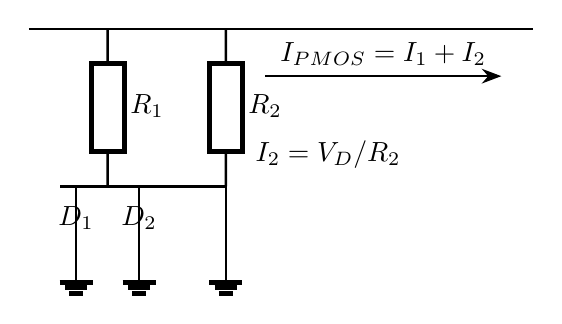
\begin{tikzpicture}[>=Stealth, line width=0.9pt]
  \draw (0,3.0) -- (6.4,3.0);
  \draw (1.0,3.0) to[resistor,l=$R_1$] (1.0,1.0);
  \draw (2.5,3.0) to[resistor,l=$R_2$] (2.5,1.0);
  \draw (0.4,1.0) -- (2.5,1.0);
  \draw (0.6,1.0) -- (0.6,0.2) node[ground] {};
  \draw (1.4,1.0) -- (1.4,0.2) node[ground] {};
  \draw (2.5,1.0) -- (2.5,0.2) node[ground] {};
  \node at (0.6,0.6) {$D_1$};
  \node at (1.4,0.6) {$D_2$};
  \draw[->] (3.0,2.4) -- (6.0,2.4) node[midway,above] {$I_{PMOS}=I_1+I_2$};
  \node at (3.8,1.4) {$I_2=V_D/R_2$};
\end{tikzpicture}
=======
../cictikz/src/cictikz/data/tex/cictikz_preamble.tex

% PTAT core (as l3_ptat) plus a unity-gain buffer that puts the diode voltage
% across R2, giving a CTAT current alongside the PTAT one. Combining the two in
% the right proportion cancels the temperature dependence.
%
% Polarity of the first OTA is corrected here as in l3_ptat: the source artwork
% marks + on the left input, but + belongs on the right for the loop to settle.

\begin{circuitikz}[american, thick, transform shape, circuit ee IEC]

  ../cictikz/src/cictikz/data/tex/cictikz_lib.tex

  \def\xl{0}
  \def\xr{\grid*2.5}
  \def\pdlevel{5}

  % ---- PTAT core ----
  \node[pnp, anchor=C] (Q1) at (\xl, 0) {};
  \draw (Q1.C) -- ++(0,-0.2) \vground;
  \draw (Q1.B) |- (Q1.C);

  \node[pnp, anchor=C, label=right:${\times N}$] (Q2) at (\xr, 0) {};
  \draw (Q2.C) -- ++(0,-0.2)\vground;
  \draw (Q2.B) |- (Q2.C);

  \draw (Q2.E) \vresistor{$R_{1}$};

  \coordinate (mp1drain) at (\xl, \pdlevel);
  \coordinate (mp2drain) at (\xr, \pdlevel);

  \def\xota{-\grid*1.5}
  \def\yota{ 3}
  \begin{scope}[xscale=-1]
  \begin{scope}[rotate around={90:(\xota,\yota)}]
    \draw (\xota, \yota) \cicOtaSSWP{}{};
    \coordinate (otaRight) at ($(\xota,\yota)+(0.5,0)$);
    \coordinate (otaLeft)  at ($(\xota,\yota)+(0.5,-\grid/2)$);
  \end{scope}
  \end{scope}
  \node at ($(otaRight)+(0,0.3)$) {$+$};
  \node at ($(otaLeft)+(0,0.3)$)  {$-$};

  \draw (cicOtaS_inp) -| (mp2drain);
  \draw (cicOtaS_inn) -| (mp1drain);
  \draw (cicOtaS_inn) -| (Q1.E);

  \draw (mp1drain) \lvmpmos{MP1}{};
  \draw (MP1.source) \vsupply;
  \draw (mp2drain) \lvpmos{MP2}{};
  \draw (MP2.source) \vsupply;

  \draw (cicOtaS_out) |- (MP1.gate);
  \draw (MP1.gate) -- (MP2.gate);

  % Short, and kept above the buffer tap wire at \ybuf.
  \draw[->] (\xr+0.9,\pdlevel-0.05) -- ++(0,-0.65);

  % ---- Buffer: senses the xN branch node, drives R2 ----
  % Drawn unrotated, so the macro's own +/- labels are upright and can be
  % passed in directly.
  \def\xbuf{6.4}
  \def\ybuf{4.0}
  \draw (\xbuf,\ybuf) \cicOtaSSWP{$+$}{$-$};

  % Tap the branch above R1 and take it to the non-inverting input.
  \draw (\xr,\ybuf) -- (\xbuf,\ybuf);
  \fill (\xr,\ybuf) circle (0.06);

  % Output down through R2 to ground, with the follower feedback tapped off it.
  \coordinate (obuf) at (\xbuf+3.2,\ybuf-0.4);
  \draw (cicOtaS_out) -- (obuf);
  \draw (\xbuf+3.2,0.6) \vresistor{$R_{2}$};
  \draw (resEnd) -- (obuf);
  \draw (\xbuf+3.2,0.6) -- ++(0,-0.4) \vground;

  \draw (\xbuf+3.2,2.6) -- (\xbuf,2.6) -- (cicOtaS_inn);
  \fill (\xbuf+3.2,2.6) circle (0.06);

  \draw[->] (\xbuf+4.0,2.3) -- ++(0,-0.9);

\end{circuitikz}
>>>>>>> 7a1064c0dd01972bf43e2231489f230bb3bf92cf
\end{document}
